% vim: set tw=78 sts=2 sw=2 ts=8 aw et:
\documentclass{so.cs.pub.ro}

\usepackage{code/highlight}

\title[Laborator 6]{Laborator 6}
\subtitle{Memoria virtuală}

\begin{document}

\frame{\titlepage}

% Titlul unui frame se specifică fie în acolade, imediat după \begin{frame}, fie
% folosind \frametitle
\begin{frame}{Memoria virtuală(1)}
\begin{columns}
\begin{column}{0.55\textwidth}
\begin{itemize}
  \item Mecanism folosit implicit..
  \begin{itemize}
    \vspace{0.4cm}
    \item de către nucleul sistemului de operare pentru a implementa o politică eficientă de gestiune a memoriei
    \vspace{0.4cm}
    \item ce astfel de optimizări cunoaşteţi?
  \end{itemize}
\end{itemize}
\end{column}
\begin{column}{0.45\textwidth}
\framebox{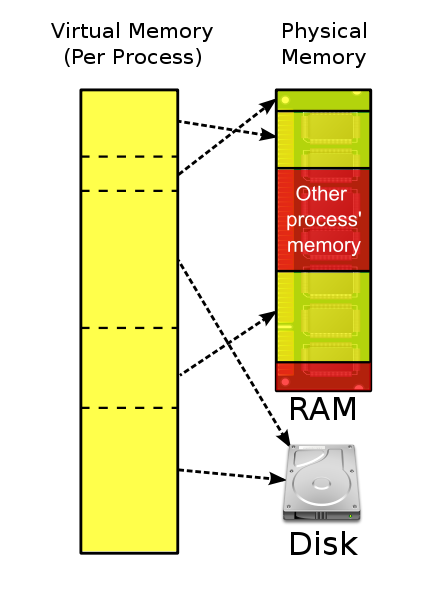
\includegraphics[height=2.5in]{code/VM.png}}
\vspace{0.2cm}
\fontsize{6}{6}\selectfont imagine preluată de pe wikipedia.org
\end{column}
\end{columns}
\end{frame}

\begin{frame}{Memoria virtuală(2)}
\begin{itemize}
  \item .. dar şi explicit, pentru a mapa în spaţiul de adresă al unui proces:
  \begin{itemize}
    \item fişiere
    \item memorie
    \item dispozitive
  \end{itemize}
\end{itemize}
\begin{itemize}
  \item Mapare fişiere
  \begin{itemize}
    \item memorie partajată
    \item paginare la cerere
    \item biblioteci partajate
  \end{itemize}
\end{itemize}
\begin{itemize}
  \item Mapare memorie
  \begin{itemize}
    \item pentru alocarea unei cantităţi mari de memorie
  \end{itemize}
\end{itemize}
\begin{itemize}
  \item Mapare dispozitive
  \begin{itemize}
    \item acces direct la memoria dispozitivului
    \item când ar putea fi necesar?
  \end{itemize}
\end{itemize}
\end{frame}

\begin{frame}{Mapare fişiere şi memorie - Linux(1)}
\begin{itemize}
  \item Accesare fişier similar cu un vector
  \vspace{0.4cm}
  \item Mapările pot depăşi dimensiunea memoriei fizice
  \vspace{0.4cm}
  \item Nu pot fi mapate dispozitive cu acces secvenţial (socket-uri, pipe-uri)
  \vspace{0.4cm}
  \item Unitate: pagina (număr întreg, alinieri)
  \vspace{0.4cm}
  \item Familia de funcţii mmap(2)
\end{itemize}
\end{frame}

\begin{frame}{Mapare fişiere şi memorie - Linux(2)}
\begin{itemize}
  \item mmap/munmap
\end{itemize}
\center{\framebox{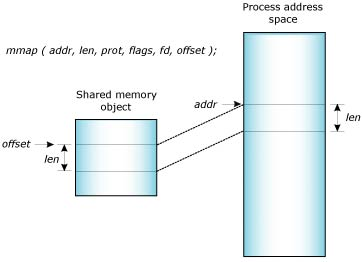
\includegraphics[height=1.3in]{code/mmap.jpg}}}
\begin{itemize}
  \item addr poate fi NULL
  \item prot: PROT_READ, PROT_WRITE, PROT_EXEC, PROT_NONE
  \item flags: MAP_PRIVATE, MAP_SHARED, MAP_FIXED, MAP_LOCKED, MAP_ANONYMOUS (pt mapare memorie)
  \item mapare memorie: ignoră fd şi offset
\end{itemize}
\begin{itemize}
  \item msync - sincronizare explicită fişier cu maparea din memorie
\end{itemize}
\end{frame}

\begin{frame}{Mapare fişiere - Windows}
\begin{itemize}
  \item CreateFileMapping/OpenFileMapping
  \begin{itemize}
    \item primeşte HANDLE fişier
    \item tip mapare: PAGE_READONLY, PAGE_READWRITE, PAGE_WRITECOPY
  \end{itemize}
  \vspace{0.3cm}
  \item MapViewOfFile
  \begin{itemize}
    \item primeşte HANDLE FileMapping
    \item mod acces: FILE_MAP_READ, FILE_MAP_WRITE, FILE_MAP_COPY
  \end{itemize}
  \vspace{0.3cm}
  \item UnmapMapViewOfFile
\end{itemize}
\end{frame}

\begin{frame}{Mapare memorie - Windows}
\begin{itemize}
  \item VirtualAlloc/VirtualAllocEx
  \begin{itemize}
    \item tip operaţie: MEM_RESERVE, MEM_COMMIT, MEM_RESET
    \item lpAddress poate fi NULL; multiplu de 4KB pentru alocare şi 64KB pentru rezervare
  \end{itemize}
  \vspace{0.3cm}
  \item VirtualFree/VirtualFreeEx
  \begin{itemize}
    \item tip operaţie: MEM_DECOMMIT, MEM_RELEASE
  \end{itemize}
  \vspace{0.3cm}
  \item Interogarea zonelor mapate VirtualQuery/VirtualQueryEx
  \begin{itemize}
    \item adresa de start a zonei, protecţie, dimensiune
    \item struct _MEMORY_BASIC_INFORMATION
  \end{itemize}
\end{itemize}
\end{frame}

\begin{frame}{Excepţii.Schimbarea protecţiei unei zone mapate}
\begin{itemize}
  \item Accese la memorie nonconforme cu drepturile
  \begin{itemize}
    \item Linux - generează semnale SIGBUS, SIGSEGV
    \begin{itemize}
      \item sigaction, siginfo_t
    \end{itemize}
    \vspace{0.3cm}
    \item Windows - generează excepţii
    \begin{itemize}
      \item AddVectoredExceptionHandler, VectoredHandler
    \end{itemize}
  \end{itemize}
  \vspace{0.5cm}
  \item Linux - mprotect
  \begin{itemize}
    \item acces: PROT_READ, PROT_WRITE, PROT_EXEC, PROT_NONE
    \item adresa multiplu de dimensiunea unei pagini
  \end{itemize}
  \vspace{0.3cm}
  \item Windows - VirtualProtect/VirtualProtectEx
  \begin{itemize}
    \item pt regiuni alocate cu VirtualAlloc/VirtualAllocEx folosind MEM_RESERVE
  \end{itemize}
\end{itemize}
\end{frame}

\begin{frame}{Blocarea paginării}
\begin{itemize}
  \item Utilă pentru procese care trebuie să execute anumite acţiuni la momente de timp bine determinate
  \vspace{0.2cm}
  \item Nu se va mai face swap out - accesele ulterioare nu mai produc page fault
  \vspace{0.5cm}
  \item Linux
  \begin{itemize}
    \item mlock
    \item mlockall
    \begin{itemize}
      \item flags: MCL_CURRENT, MCL_FUTURE
    \end{itemize}
    \item munlock/munlockall
  \end{itemize}
  \vspace{0.5cm}
  \item Windows
  \begin{itemize}
    \item VirtualLock/VirtualLockEx
    \begin{itemize}
      \item rezultat: TRUE succes, FALSE altfel
    \end{itemize}
    \item VirtualUnlock/VirtualUnlockEx
  \end{itemize}
\end{itemize}
\end{frame}

%\begin{frame}{Întrebări}
%\begin{itemize}
%\item Câte page fault-uri se pot genera în urma execuției următorului cod: \\
%char *a = malloc(5000);\\
%memset(a, 0, 5000);
%\item De ce este apelul malloc mai rapid decât calloc?
%\item Pot două procese să partajeze o pagină virtuală?
%\item Dacă un access la memorie durează 50 ns, cât durează execuția următorului cod:\\
%int a[1030]; \\
%a[0] = a[1029] = 42;\\
%Presupunem că avem un sistem cu paginare simplă.
%\end{itemize}
%\end{frame}

\end{document}
